\textbf{\textit{The Models}}---
Let us start by discussing aforementioned new physics models in more detail.
The first scenario under consideration is active-to-sterile neutrino transition magnetic moment described by \cite{Magill:2018jla,Brdar:2020quo,Brdar:2023tmi}
\begin{align}
    \mathcal{L} \supset \sum_\alpha d_\alpha \bar{N}\sigma_{\mu\nu} \nu^{\alpha} F^{\mu\nu}-\frac{M_N}{2} \bar{N}^c N + \text{h.c.}\,,
    \label{eq:Lag}
\end{align}
where $\nu^{\alpha}$ and $N$ represent active and sterile neutrinos, respectively. Further, $F^{\mu\nu}$ is the field strength tensor of the electromagnetic field and $d_\alpha$ is the dimensionful coefficient of this dimension-5 term and $M_N$ is sterile neutrino mass. We will abbreviate $d_\alpha \equiv d$ given that we assume flavor universal interaction. The dominant production channels for $N$ inside the SN are $\nu e^- \to \nu e^-$ at lower energies and $\nu \gamma \to N$ for larger active neutrino energies. Both processes occur due to the interaction term in \cref{eq:Lag}; after $N$ are produced, they decay to active neutrinos and photons which is again realized through the same term in the Lagrangian, with the decay width for $N\to\nu\gamma$ given by $\Gamma_N = 6d^2 M_N^3/4 \pi$ \cite{Plestid:2020vqf}. 

The second model that will be analyzed in this work is the Majoron model from \cite{Fiorillo:2022cdq}. The relevant part of the Lagrangian reads
\begin{align}
\mathcal{L} \supset -\frac{g_{\alpha\beta}}{2} \nu_\alpha \nu_\beta \phi - M_\phi \phi\phi^* + \text{h.c.}\,,
\end{align}
where $M_\phi$ is the Majoron mass and $g$ parametrizes interaction strength between $\phi$ and neutrinos. As in the previous model, we assume flavor universal interaction, hence we abbreviate $g_{\alpha\beta}\equiv g$. Majorons are produced from neutrino coalescence in the star and then subsequently decay to a pair of neutrinos with the total decay width to all flavor of neutrinos given by $\Gamma_\phi = 3g^2 m_\phi/16 \pi$, and as a result, BSM neutrino flux is produced. 


%The differential number of sterile neutrinos $\mathcal{N}_s$ produced per unit time $t$ at position $r$ is \cite{Arguelles:2016uwb}
%\begin{align}
%\frac{1}{4\pi r^2}\frac{\partial^2}{\partial r\partial t}\left(\frac{d\mathcal{N}_s}{dE_N}\right)= \sigma n_\nu \frac{d n}{dE}\,.
%\label{eq:simplified}
%\end{align}
%where $\sigma n_\nu$ is the interaction rate for the production process with $n_\nu$ being the number densities of the neutrino. $n$ is the number density of electron (neutrino) for sterile neutrion $N$ (Majoron $\phi$) production. 
Using data simulated by the Garching group for an $8.8 M_\odot$ progenitor star \cite{Huedepohl2010}, we obtained the fluxes of sterile neutrino $N$ and Majoron $\phi$, and produced the cooling limit as depicted in Fig. \cref{fig:exclusion}. The results are in agreement with those obtained in literature \cite{Fiorillo:2022cdq, Brdar:2023tmi}.
%, with the  ``cooling'' bound depicted in \cref{fig:exclusion} (gray region).
%Requiring the total energy carried away by $N$ to be less than $10\%$ of the total available neutrino energy leads to the  ``cooling'' bound depicted in \cref{fig:exclusion} (gray region). Our estimate is in agreement with the one obtained in \cite{Fiorillo:2022cdq, Brdar:2023tmi}. 
As we are interested in cases where the coupling strength is below the cooling limit, these new states once produced in the SN core will stream out without further interacting with SN plasma before decaying.
 For a given emission angle $\alpha$ of daughter neutrino relative to the direction of mother particle, and the angle $\theta$ at which the daughter neutrino arrives at the Earth, the time delay $\Delta t$, the arrival time of the daughter $\gamma$/$\nu$ relative to that of the neutrinos produced in the explosion via SM processes, is \cite{Jaeckel:2017tud}
\begin{align}
    \Delta t = L_1/\beta + D_{\rm SN} \cos\theta-L_1 \cos\alpha -D_{\rm SN}\,,
    \label{eq:deltat}
\end{align}
with $D_{\rm SN}$ the distance between the SN and the Earth, and $L_1$ the distance mother particles propagated before decaying.
The flux of daughter $\nu$ is obtained by considering decays that only occur at $R^{\gamma/\nu}_{\rm SN}\leq L_1 \leq L^{\rm max}_1$. As the smallest decay distance beyond which the daughter neutrino can escape the explosion unperturbed, we take $R^{\nu}_{\rm SN} = \unit[30]{km}$.
$L^{\rm max}_1$ corresponds to the distance $L_1$ with the largest time delay $\delta t = \unit[100]{s}$ while larger values of $\delta t$ do not affect the limits obtained. For the time delay bounded by $\delta t = \unit[100]{s}$, $\theta < 5^\circ$ \cite{Brdar:2023tmi}. We show the fluxes of daughter neutrino in comparison to the standard neutrino flux in Fig. \cref{fig:fluxes}.

\begin{figure}[t!]
    \centering
    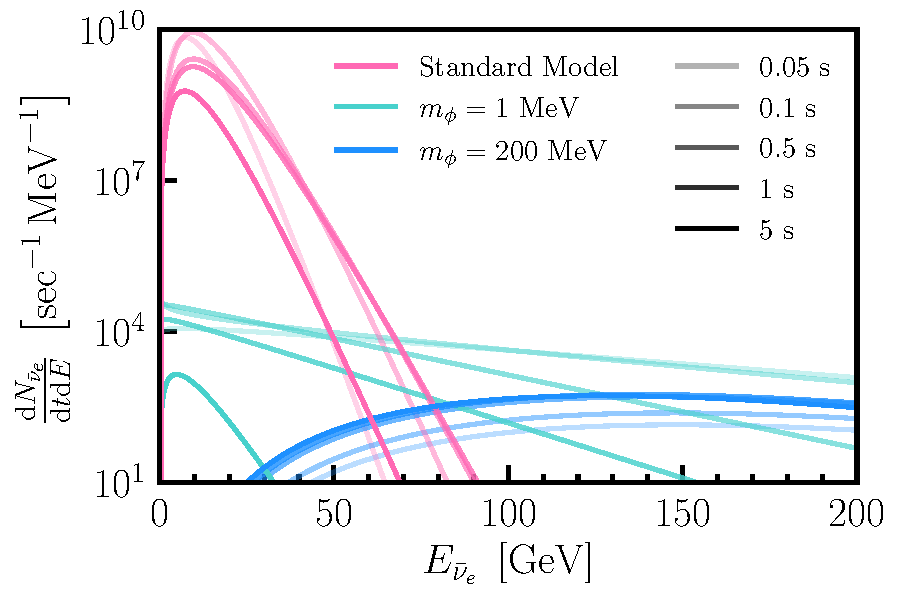
\includegraphics[width=0.47\textwidth]{figures/majoran_fluxes.pdf}
    \caption{\textbf{\textit{Neutrino flux from Standard Model production and two majoran hypotheses.}}
    Jeff needs to write here.
    }
    \label{fig:fluxes}
\end{figure}